\documentclass{beamer}
\usepackage[utf8]{inputenc}

\usetheme{Madrid}
\usecolortheme{default}
\usepackage{amsmath,amssymb,amsfonts,amsthm}
\usepackage{mathtools}
\usepackage{txfonts}
\usepackage{tkz-euclide}
\usepackage{listings}
\usepackage{adjustbox}
\usepackage{tfrupee}
\usepackage{array}
\usepackage{gensymb}
\usepackage{tabularx}
\usepackage{gvv}
\usepackage{lmodern}
\usepackage{circuitikz}
\usepackage{tikz}
\lstset{literate={·}{{$\cdot$}}1 {λ}{{$\lambda$}}1 {→}{{$\to$}}1}
\usepackage{graphicx}

\setbeamertemplate{page number in head/foot}[totalframenumber]

\usepackage{tcolorbox}
\tcbuselibrary{minted,breakable,xparse,skins}

\definecolor{bg}{gray}{0.95}
\DeclareTCBListing{mintedbox}{O{}m!O{}}{%
  breakable=true,
  listing engine=minted,
  listing only,
  minted language=#2,
  minted style=default,
  minted options={%
    linenos,
    gobble=0,
    breaklines=true,
    breakafter=,,
    fontsize=\small,
    numbersep=8pt,
    #1},
  boxsep=0pt,
  left skip=0pt,
  right skip=0pt,
  left=25pt,
  right=0pt,
  top=3pt,
  bottom=3pt,
  arc=5pt,
  leftrule=0pt,
  rightrule=0pt,
  bottomrule=2pt,
  toprule=2pt,
  colback=bg,
  colframe=orange!70,
  enhanced,
  overlay={%
    \begin{tcbclipinterior}
    \fill[orange!20!white] (frame.south west) rectangle ([xshift=20pt]frame.north west);
    \end{tcbclipinterior}},
  #3,
}
\lstset{
    language=C,
    basicstyle=\ttfamily\small,
    keywordstyle=\color{blue},
    stringstyle=\color{orange},
    commentstyle=\color{green!60!black},
    numbers=left,
    numberstyle=\tiny\color{gray},
    breaklines=true,
    showstringspaces=false,
}

\title{12.235}
\date{September 30, 2025}
\author{Bhargav - EE25BTECH11013}

\begin{document}

\frame{\titlepage}

\begin{frame}{Question}
\textbf{Question}: \\
A system of equations represented as
\begin{align}
\myvec{1 & -1 & 2 \\ 2 & 1 & 4 \\ 1 & 3 & 1}\myvec{x_1 \\ x_2 \\ x_3} = \myvec{4 \\ y \\ 3} is,
\end{align}
\begin{enumerate}
\item consistent and has a unique solution
\item inconsistent and has no solution
\item consistent and infinite solution
\item inconsistent and has unique solution
\end{enumerate}
\end{frame}
\begin{frame}{Solution}
This can be represented as an augmented matrix and can be solved by using Gaussian elimination.
\begin{align}
\augvec{3}{1}{1 & -1 & 2 & 4\\ 2 & 1 & 4 & y\\ 1 & 3 & 1 & 3} \xleftrightarrow[R_3 \leftarrow R_3 - R_1]{R_2 \leftarrow R_2 - 2R_1}\augvec{3}{1}{1 & -1 & 2 & 4 \\ 0 & 3 & 0 & y-8 \\ 0 & 4 & -1 & -1}
\end{align}
\begin{align}
\xleftrightarrow[R_3 \leftarrow R_3 - 4R_2]{R_2 \leftarrow \frac{R_2}{3}} \augvec{3}{1}{1 & -1 & 2 & 4\\ 0 & 1 & 0 & \frac{y-8}{3} \\ 0 & 0 & -1 & \frac{29-4y}{3}} \xleftrightarrow[R_1 \leftarrow R_1 - 2R_3]{R_3 \leftarrow -R_3}
\end{align}
\begin{align}
\augvec{3}{1}{1 & -1 & 0 & \frac{70- 8y}{3} \\ 0 & 1 & 0 & \frac{y-8}{3}\\ 0 & 0 & 1 & \frac{4y-29}{3}} \xleftrightarrow{R_1 \leftarrow R_1 + R_2} \augvec{3}{1}{1 & 0 & 0 & \frac{62 - 7y}{3} \\ 0 & 1 & 0 & \frac{y-8}{3} \\ 0 & 0 & 1 & \frac{4y - 29}{3}}
\end{align}
\end{frame}

\begin{frame}{Solution}
\begin{align}
\myvec{x_1 \\ x_2 \\ x_3} = \myvec{\frac{62 - 7y}{3} \\ \frac{y-8}{3} \\ \frac{4y - 29}{3}}
\end{align}
Since $y  \in \mathbf{R}$, we can conclude that there exists a unique solution and the system of equations is consistent. \\

Option (1) is the correct answer

\end{frame}

\begin{frame}{Solution}
This can be verified by finding the point of intersection of 3 planes:\\
As an example, take $y = 8$
\begin{align}
x_1 - x_2 + 2x_3 = 4
\end{align}
\begin{align}
2x_1 + x_2 + 4x_3 = 8
\end{align}
\begin{align}
x_1 + 3x_2 + x_3 = 3
\end{align}

The point of intersection of the planes from \brak{5} is
\begin{align}
\myvec{x_1 \\ x_2 \\ x_3} = \myvec{2 \\ 0 \\ 1}
\end{align}
\end{frame}

\begin{frame}{Plot}
\begin{figure}[H]
    \centering
    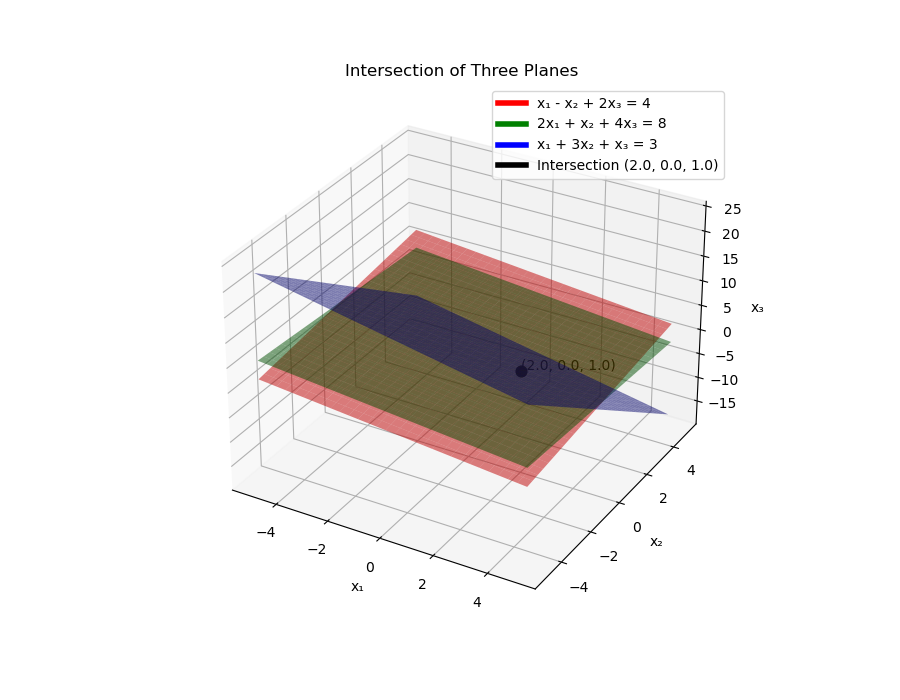
\includegraphics[height=0.5\textheight, keepaspectratio]{figs/Figure_1.png}
    \label{figure_1}
\end{figure}
\end{frame}

\begin{frame}[fragile]
    \frametitle{C Code}
    \begin{lstlisting}
#include <stdio.h>

void solve_planes(double *A, double *b, double *x) {
    double detA, det1, det2, det3;

    detA = A[0]*(A[4]*A[8] - A[5]*A[7]) -
           A[1]*(A[3]*A[8] - A[5]*A[6]) +
           A[2]*(A[3]*A[7] - A[4]*A[6]);

    if(detA == 0) {
        x[0] = x[1] = x[2] = 0;
        return;
    }

    det1 = b[0]*(A[4]*A[8] - A[5]*A[7]) -
           A[1]*(b[1]*A[8] - A[5]*b[2]) +
           A[2]*(b[1]*A[7] - A[4]*b[2]);

    \end{lstlisting}
\end{frame}
\begin{frame}[fragile]
    \frametitle{C Code}
    \begin{lstlisting}
    det2 = A[0]*(b[1]*A[8] - A[5]*b[2]) -
           b[0]*(A[3]*A[8] - A[5]*A[6]) +
           A[2]*(A[3]*b[2] - b[1]*A[6]);

    det3 = A[0]*(A[4]*b[2] - b[1]*A[7]) -
           A[1]*(A[3]*b[2] - b[1]*A[6]) +
           b[0]*(A[3]*A[7] - A[4]*A[6]);

    x[0] = det1 / detA;
    x[1] = det2 / detA;
    x[2] = det3 / detA;
}

    \end{lstlisting}
\end{frame}

\begin{frame}[fragile]
    \frametitle{Python + C Code}
    \begin{lstlisting}
import numpy as np
import ctypes
import matplotlib.pyplot as plt

# Load shared C library
lib = ctypes.CDLL("./libcode.so")

# Define argument types
lib.solve_planes.argtypes = [
    np.ctypeslib.ndpointer(dtype=np.double, ndim=1, flags="C_CONTIGUOUS"),
    np.ctypeslib.ndpointer(dtype=np.double, ndim=1, flags="C_CONTIGUOUS"),
    np.ctypeslib.ndpointer(dtype=np.double, ndim=1, flags="C_CONTIGUOUS")
]

    \end{lstlisting}
\end{frame}
\begin{frame}[fragile]
    \frametitle{Python + C Code}
    \begin{lstlisting}
# Coefficient matrix and constants
A = np.array([[1, -1, 2],
              [2,  1, 4],
              [1,  3, 1]], dtype=np.double)
b = np.array([4, 8, 3], dtype=np.double)
x = np.zeros(3, dtype=np.double)

# Call C function
lib.solve_planes(A.ravel(), b, x)
print("Point of intersection (x1, x2, x3):", x)

# --- Plotting ---
x_vals = np.linspace(-5, 5, 30)
y_vals = np.linspace(-5, 5, 30)
X, Y = np.meshgrid(x_vals, y_vals)

# Plane equations rearranged for z
Z1 = (4 - X + Y) / 2
Z2 = (8 - 2*X - Y) / 4


    \end{lstlisting}
\end{frame}
\begin{frame}[fragile]
    \frametitle{Python + C Code}
    \begin{lstlisting}
Z3 = 3 - X - 3*Y

fig = plt.figure(figsize=(9, 7))
ax = plt.axes(projection='3d')

# Plot each plane
ax.plot_surface(X, Y, Z1, alpha=0.5, color='red')
ax.plot_surface(X, Y, Z2, alpha=0.5, color='green')
ax.plot_surface(X, Y, Z3, alpha=0.5, color='blue')

# Plot intersection point
ax.scatter(x[0], x[1], x[2], color='black', s=60)
ax.text(x[0], x[1], x[2]+0.3, f'({x[0]:.1f}, {x[1]:.1f}, {x[2]:.1f})', color='black')

# Labels and title
ax.set_xlabel('x₁')
ax.set_ylabel('x₂')
ax.set_zlabel('x₃')
ax.set_title('Intersection of Three Planes')

colors = ['red', 'green', 'blue', 'black']
labels = [
    'x₁ - x₂ + 2x₃ = 4',
    '2x₁ + x₂ + 4x₃ = 8',
    'x₁ + 3x₂ + x₃ = 3',
    'Intersection (2, 0, 1)'
]

handles = [plt.Line2D([0], [0], color=c, lw=4) for c in colors]
ax.legend(handles, labels)
plt.savefig("/mnt/c/Users/bharg/Documents/backupmatrix/ee25btech11013/matgeo/12.235/figs/Figure_1.png")
plt.show()
    \end{lstlisting}
\end{frame}

\begin{frame}[fragile]
    \frametitle{Python + C Code}
    \begin{lstlisting}
colors = ['red', 'green', 'blue', 'black']
labels = [
    'x₁ - x₂ + 2x₃ = 4',
    '2x₁ + x₂ + 4x₃ = 8',
    'x₁ + 3x₂ + x₃ = 3',
    'Intersection (2, 0, 1)'
]

handles = [plt.Line2D([0], [0], color=c, lw=4) for c in colors]
ax.legend(handles, labels)
plt.savefig("/mnt/c/Users/bharg/Documents/backupmatrix/ee25btech11013/matgeo/12.235/figs/Figure_1.png")
plt.show()

    \end{lstlisting}
\end{frame}

\begin{frame}[fragile]
    \frametitle{Python Code}
    \begin{lstlisting}
import numpy as np
import matplotlib.pyplot as plt
A = np.array([[1, -1, 2],
              [2,  1, 4],
              [1,  3, 1]], dtype=float)
b = np.array([4, 8, 3], dtype=float)
x = np.linalg.solve(A, b)
print("Point of intersection (x1, x2, x3):", x)
x_vals = np.linspace(-5, 5, 30)
y_vals = np.linspace(-5, 5, 30)
X, Y = np.meshgrid(x_vals, y_vals)
# Plane equations rearranged for z
Z1 = (4 - X + Y) / 2
Z2 = (8 - 2*X - Y) / 4
Z3 = 3 - X - 3*Y

fig = plt.figure(figsize=(9, 7))
ax = fig.add_subplot(111, projection='3d')



    \end{lstlisting}
\end{frame}
\begin{frame}[fragile]
    \frametitle{Python Code}
    \begin{lstlisting}
# Plot each plane
surf1 = ax.plot_surface(X, Y, Z1, alpha=0.5, color='red')
surf2 = ax.plot_surface(X, Y, Z2, alpha=0.5, color='green')
surf3 = ax.plot_surface(X, Y, Z3, alpha=0.5, color='blue')

# Plot intersection point
ax.scatter(x[0], x[1], x[2], color='black', s=60)
ax.text(x[0], x[1], x[2]+0.3, f'({x[0]:.1f}, {x[1]:.1f}, {x[2]:.1f})', color='black')

# Labels and title
ax.set_xlabel('x₁')
ax.set_ylabel('x₂')
ax.set_zlabel('x₃')
ax.set_title('Intersection of Three Planes')


    \end{lstlisting}
\end{frame}
\begin{frame}[fragile]
    \frametitle{Python Code}
    \begin{lstlisting}

colors = ['red', 'green', 'blue', 'black']
labels = [
    'x₁ - x₂ + 2x₃ = 4',
    '2x₁ + x₂ + 4x₃ = 8',
    'x₁ + 3x₂ + x₃ = 3',
    f'Intersection ({x[0]:.1f}, {x[1]:.1f}, {x[2]:.1f})'
]
handles = [plt.Line2D([0], [0], color=c, lw=4) for c in colors]
ax.legend(handles, labels)


plt.savefig("/mnt/c/Users/bharg/Documents/backupmatrix/ee25btech11013/matgeo/12.235/figs/Figure_1.png")
plt.show()

    \end{lstlisting}
\end{frame}

\end{document}

